%%%%%%%%%%%%%%%%%%%%%%%%%%%%%%%%%%%%%%%%%
% Short Sectioned Assignment LaTeX Template Version 1.0 (5/5/12)
% This template has been downloaded from: http://www.LaTeXTemplates.com
% Original author:  Frits Wenneker (http://www.howtotex.com)
% License: CC BY-NC-SA 3.0 (http://creativecommons.org/licenses/by-nc-sa/3.0/)
%%%%%%%%%%%%%%%%%%%%%%%%%%%%%%%%%%%%%%%%%

%----------------------------------------------------------------------------------------
%	PACKAGES AND OTHER DOCUMENT CONFIGURATIONS
%----------------------------------------------------------------------------------------

\documentclass[paper=a4, fontsize=11pt]{scrartcl} % A4 paper and 11pt font size

% ---- Entrada y salida de texto -----

\usepackage[T1]{fontenc} % Use 8-bit encoding that has 256 glyphs
\usepackage[utf8]{inputenc}
%\usepackage{fourier} % Use the Adobe Utopia font for the document - comment this line to return to the LaTeX default

% ---- Idioma --------

\usepackage[spanish, es-tabla]{babel} % Selecciona el español para palabras introducidas automáticamente, p.ej. "septiembre" en la fecha y especifica que se use la palabra Tabla en vez de Cuadro

% ---- Otros paquetes ----

\usepackage{url} % ,href} %para incluir URLs e hipervínculos dentro del texto (aunque hay que instalar href)
\usepackage{amsmath,amsfonts,amsthm} % Math packages
%\usepackage{graphics,graphicx, floatrow} %para incluir imágenes y notas en las imágenes
\usepackage{graphics,graphicx, float} %para incluir imágenes y colocarlas

% Para hacer tablas comlejas
%\usepackage{multirow}
%\usepackage{threeparttable}

%\usepackage{sectsty} % Allows customizing section commands
%\allsectionsfont{\centering \normalfont\scshape} % Make all sections centered, the default font and small caps

\usepackage{fancyhdr} % Custom headers and footers
\pagestyle{fancyplain} % Makes all pages in the document conform to the custom headers and footers
\usepackage{eurosym} % Para poder añadir el símbolo del euro
\fancyhead{} % No page header - if you want one, create it in the same way as the footers below
\fancyfoot[L]{} % Empty left footer
\fancyfoot[C]{} % Empty center footer
\fancyfoot[R]{\thepage} % Page numbering for right footer
\renewcommand{\headrulewidth}{0pt} % Remove header underlines
\renewcommand{\footrulewidth}{0pt} % Remove footer underlines
\setlength{\headheight}{13.6pt} % Customize the height of the header

\numberwithin{equation}{section} % Number equations within sections (i.e. 1.1, 1.2, 2.1, 2.2 instead of 1, 2, 3, 4)
\numberwithin{figure}{section} % Number figures within sections (i.e. 1.1, 1.2, 2.1, 2.2 instead of 1, 2, 3, 4)
\numberwithin{table}{section} % Number tables within sections (i.e. 1.1, 1.2, 2.1, 2.2 instead of 1, 2, 3, 4)

\setlength\parindent{0pt} % Removes all indentation from paragraphs - comment this line for an assignment with lots of text

\newcommand{\horrule}[1]{\rule{\linewidth}{#1}} % Create horizontal rule command with 1 argument of height


%----------------------------------------------------------------------------------------
%	TÍTULO Y DATOS DEL ALUMNO
%----------------------------------------------------------------------------------------

\title{	
\normalfont \normalsize 
\textsc{\textbf{Ingeniería de Servidores} \\ Doble Grado en Ingeniería Informática y Matemáticas \\ Universidad de Granada} \\ [25pt] % Your university, school and/or department name(s)
\horrule{0.5pt} \\[0.4cm] % Thin top horizontal rule
\huge Práctica 4: Benchmarking y Ajuste del Sistema \\ % The assignment title
\horrule{2pt} \\[0.5cm] % Thick bottom horizontal rule
}

\author{Alberto Jesús Durán López} % Nombre y apellidos

\date{\normalsize\today} % Incluye la fecha actual

%----------------------------------------------------------------------------------------
% DOCUMENTO
%----------------------------------------------------------------------------------------

\begin{document}

\maketitle % Muestra el Título

%\newpage %inserta un salto de página

%\tableofcontents % para generar el índice de contenidos

%\listoffigures

% \listoftables

\newpage

En esta práctica utilizaremos una serie de benchmarks para medir el rendimiento de 
nuestros servicios. Empezaremos con Phoronix.

\section{Phoronix}

Phoronix es una plataforma que permite ejecutar un conjunto de benchmarks bajo la agrupación de openbenchmarking.org. Tras conocer los benchmarks, podemos instalarlos y ejecutarlos. También podemos hacer uso de su interfaz gráfica y realizar un seguimiento con Zabbix.

\subsection{Instalación}
-Instalamos phoronix: \\
\# \textit{sudo apt-get install phoronix-test-suite} \\


Ahora comprobamos los tests disponibles de phoronix: \\
\# \textit{phoronix-test-suite list-available-tests} \\


\begin{figure}[h]
	\centering
	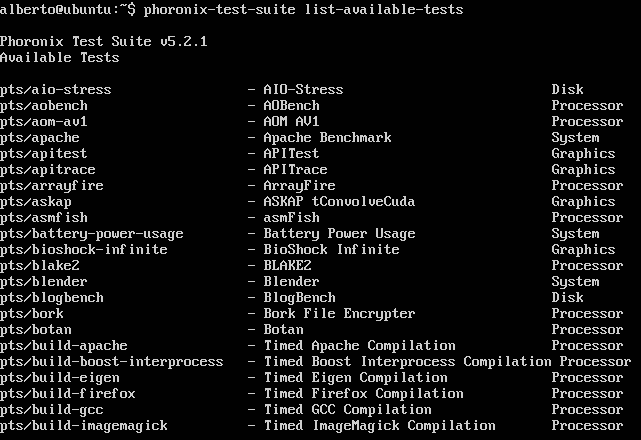
\includegraphics[scale=0.5]{images/available.png}
	\caption{Phoronix, tests disponibles}
\end{figure}


Para probar el benchmark que queramos, tendremos que instalarlo y después ejecutarlo. \\
\newpage
En nuestro caso probaremos con \textbf{sudokut}\\ 
\# \textit{phoronix-test-suite install pts/sudokut} \\
\# \textit{phoronix-test-suite run pts/sudokut} \\


\begin{figure}[h]
	\centering
	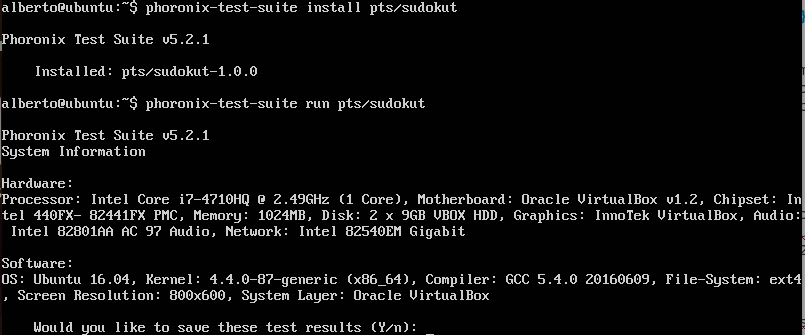
\includegraphics[scale=0.5]{images/install.png}
	\caption{Instalando y ejecutando benchmark}
\end{figure}


Por otro lado, Phoronix nos ofrece la posibilidad de probar los benchmark con 
su interfaz gráfica. Para ello nos conectamos por ssh del host a la máquina de Ubuntu Server:\\
\# \textit{ssh -X -p 22022 alberto@192.168.56.105} \\
\begin{figure}[h]
	\centering
	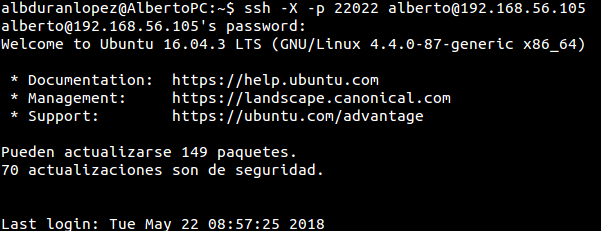
\includegraphics[scale=0.5]{images/ssh.png}
	\caption{Conexión por ssh}
\end{figure}

\newpage
Corremos la interfaz con el siguiente comando. Se nos abrirá una pestaña de firefox con la
interfaz \\
\# \textit{phoronix-test-suite gui} 

\begin{figure}[h]
	\centering
	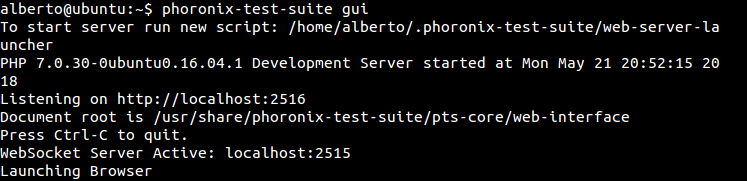
\includegraphics[scale=0.5]{images/gui.png}
	\caption{Phoronix GUI}
\end{figure}


Desde la interfaz gráfica, nos dirigimos a \textit{Available tests}, buscaremos sudokut y lo probaremos:

\begin{figure}[h]
	\centering
	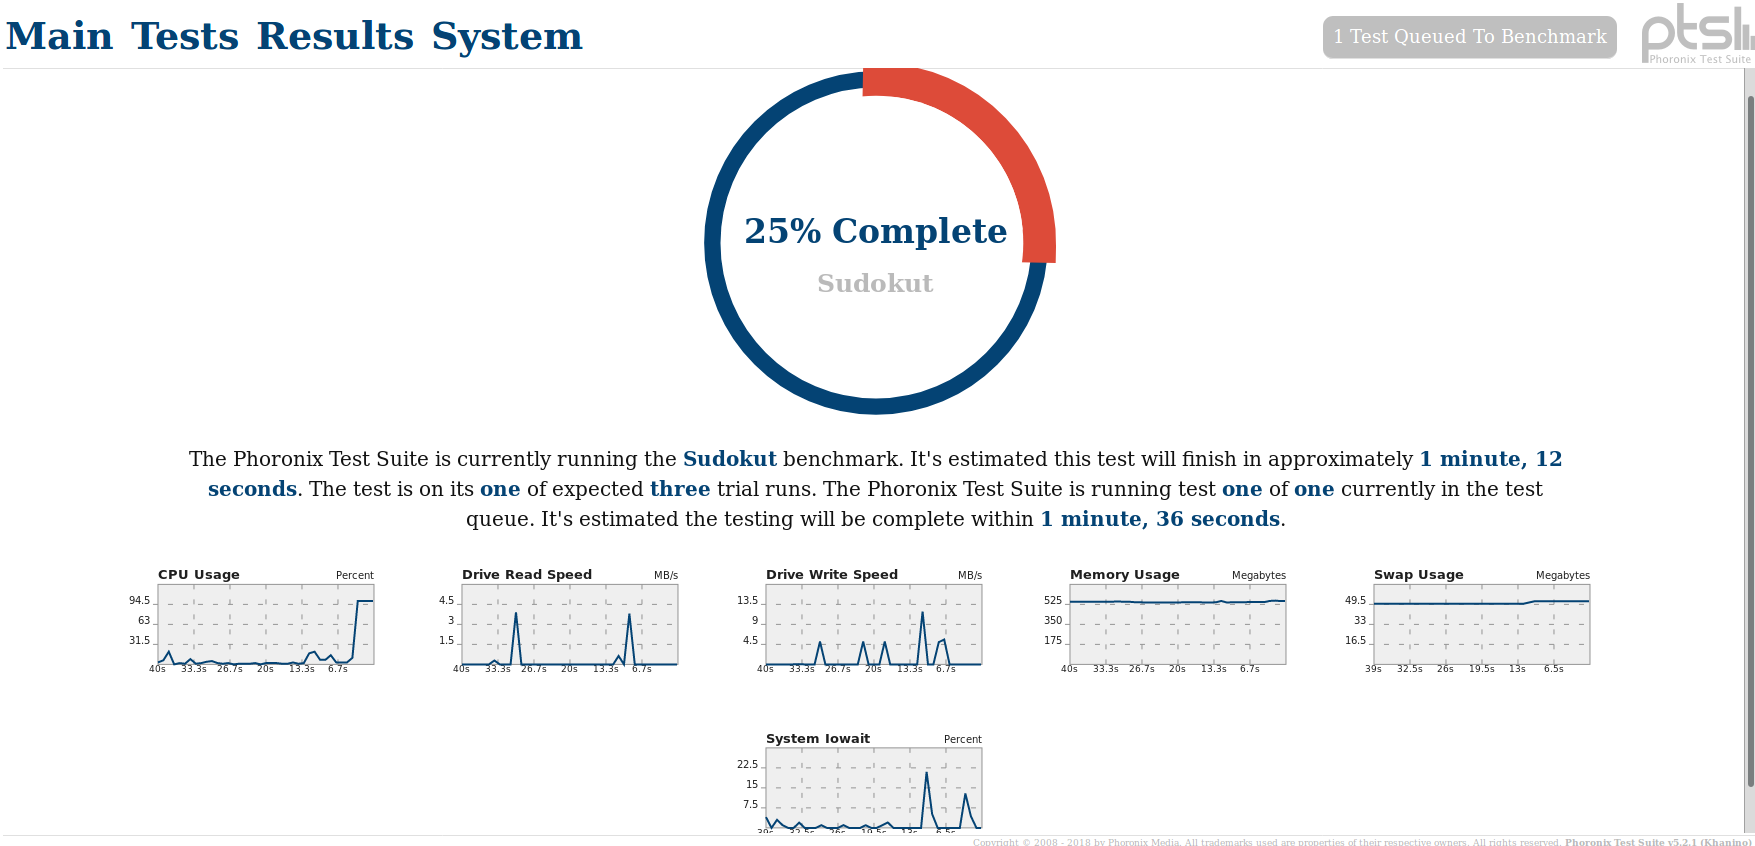
\includegraphics[scale=0.25]{images/sudokut.png}
	\caption{Sudokut en interfaz gráfica}
\end{figure}

\newpage
Ahora bien, probaremos algunos tests que nos ofrece phoronix, cabe destacar que podremos usar zabbix y monitorizar el proceso para comprobar que todo se está realizando correctamente. En la siguiente imagen podemos ver como a la hora de ejecutar un benchmark se genera un pico ya que la GPU deja de estar en estado ocioso y aumenta el tiempo de la CPU de entrada y salidas:

\begin{figure}[h]
	\centering
	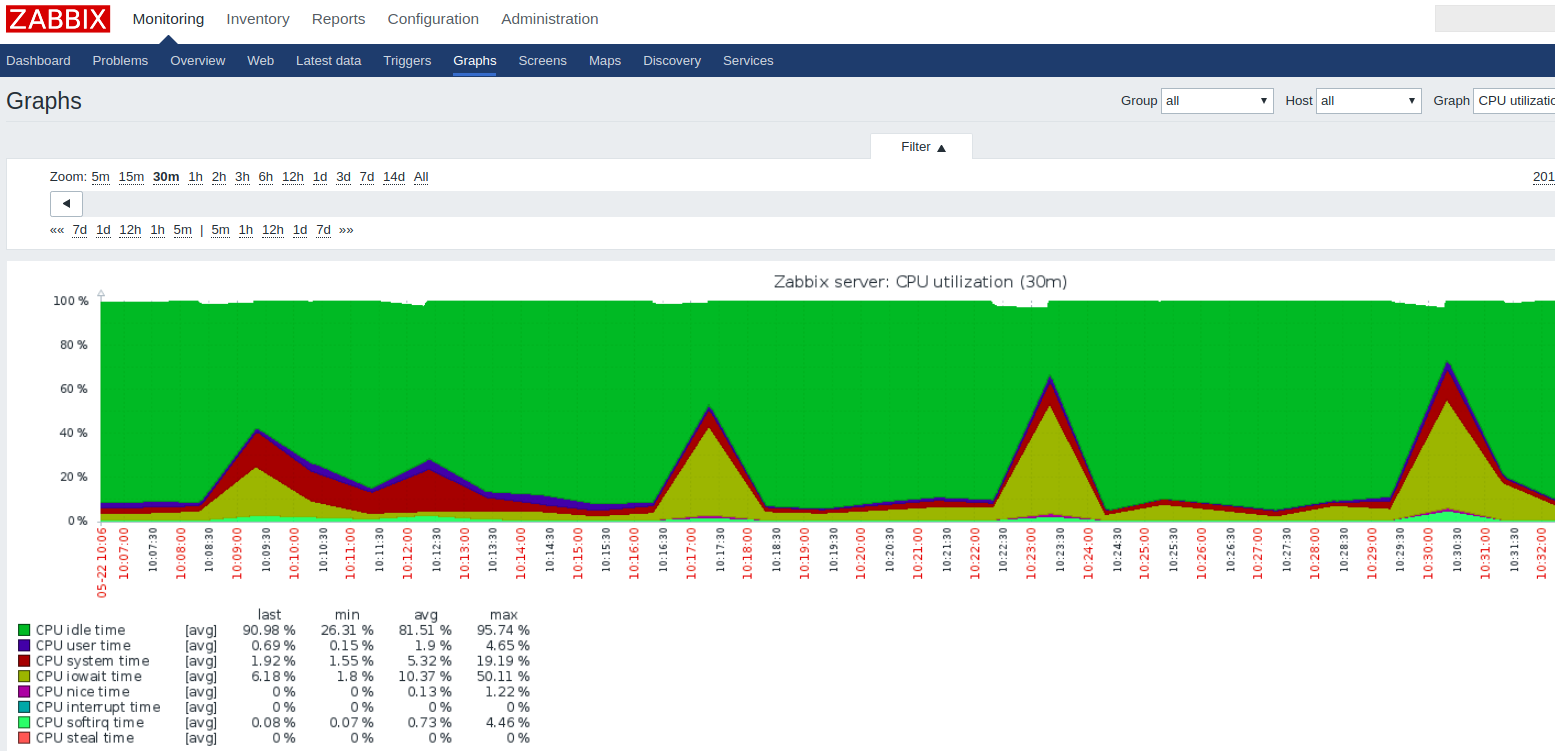
\includegraphics[scale=0.25]{images/zabbix.png}
	\caption{Sudokut en interfaz gráfica}
\end{figure}

Para ver los resultados de los diferentes benchmarks elegidos, podremos verlos desde el modo gráfico que nos ofrece phoronix o desde la propia terminal de ubuntu server:


\begin{figure}[h]
	\centering
	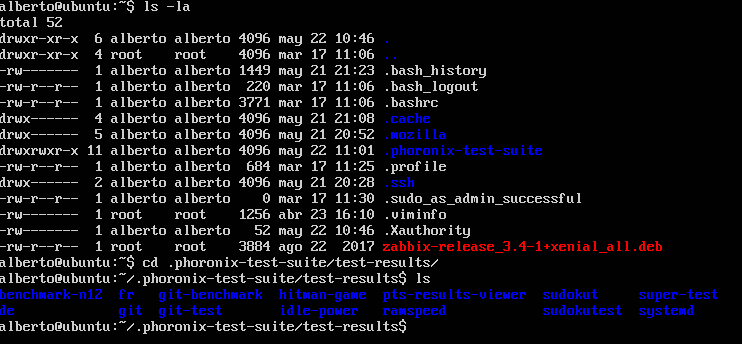
\includegraphics[scale=0.40]{images/tests.png}
	\caption{Test results}
\end{figure}

\newpage

Ejecutamos varios benchmarks y nos familiarizamos con el entorno.

A continuación se muestran los resultados del benchmark \textit{Systemd}, en este caso ha tardado 60079 milisegundos (ms) de media entre los tests que ha hecho.


\begin{figure}[h]
	\centering
	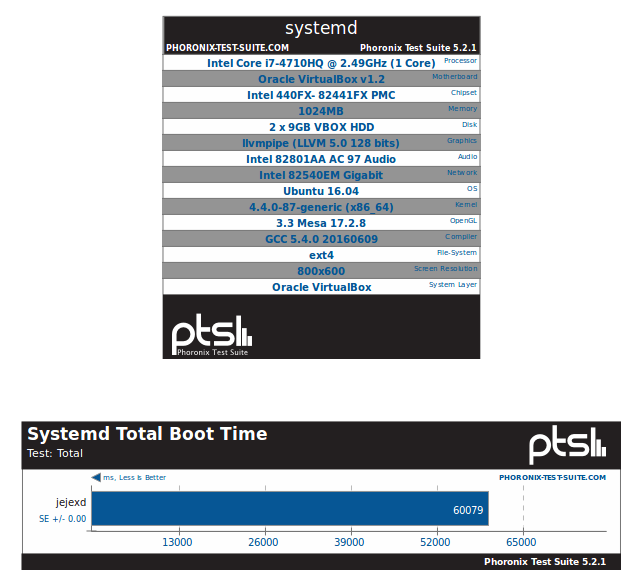
\includegraphics[scale=0.35]{images/terminal.png}
	\caption{Test results, systemd}
\end{figure}

Resultados de Sudokut desde la terminal. Se ejecuta el benchmark 3 veces y se muestra la media en segundos

\begin{figure}[h]
	\centering
	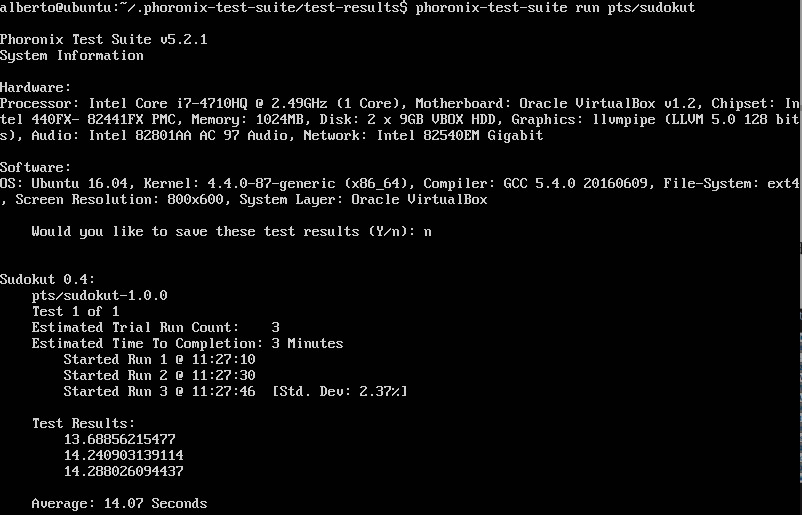
\includegraphics[scale=0.35]{images/fotito.png}
	\caption{Test results}
\end{figure}


\newpage

En total, hemos realizado varios benchmark con phoronix, entre ellos \textit{sudokut} y \textit{ramspeed}. Para saber cual es la métrica usada en cada benchmark, podemos verla con: \\
\# \textit{phoronix-test-suite info pts/sudokut} 

\begin{figure}[h]
	\centering
	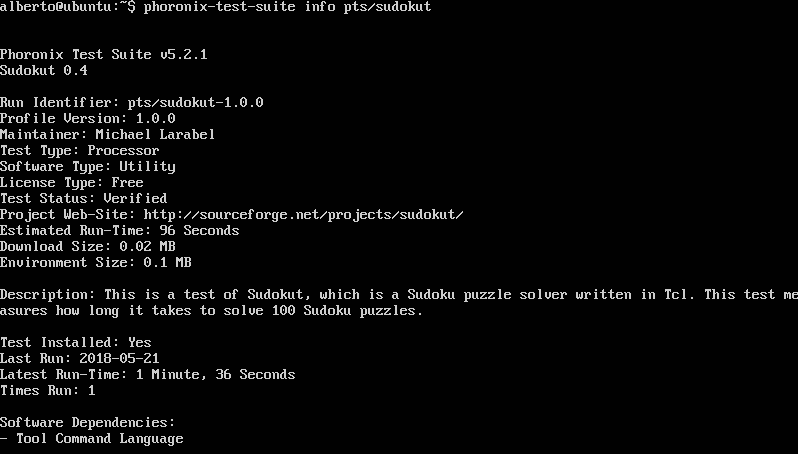
\includegraphics[scale=0.4]{images/sudok.png}
	\caption{Sudokut test}
\end{figure}

\# \textit{phoronix-test-suite info pts/ramspeed} 


\begin{figure}[h]
	\centering
	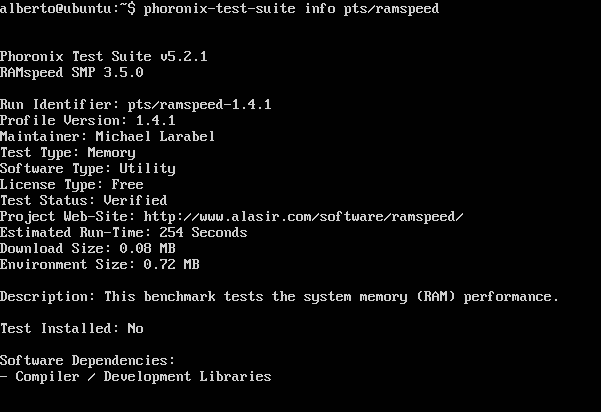
\includegraphics[scale=0.41]{images/rams.png}
	\caption{Ramspeed test}
	
\end{figure}

Por tanto, \textit{sudokut} mide el tiempo que se tarda en resolver 100 puzzles del juego sudoku mientras que \textit{ramspeed} comprueba el rendimiento de la RAM.


\newpage
\section{Ab}

Apache BenchMark es uno de los benchmarks más populares para servidores web, cuyo comando es ab.
Su misión es mostrar cuantas peticiones por segundo el servidor de HTTP (puede ser Apache, Nginx, IIS o cualquier otro) es capaz de servir.

Para consultar todas las opciones de Apache BenchMark podemos hacerlo con man: \\
\# \textit{man ab} 




Para iniciar dicho benchmark, lo hacemos con el siguiente comando: \\
\# \textit{ab -n 10000 -c 10} \\

La opción -n nos indica el número de peticiones a enviar al servidor mientras que la opción -c sirve para indicar la concurrencia, es decir, el número de peticiones a servir concurrentemente.


\begin{itemize}
	\item Benchmark sobre UbuntuServer:
	\begin{figure}[h]
		\centering
		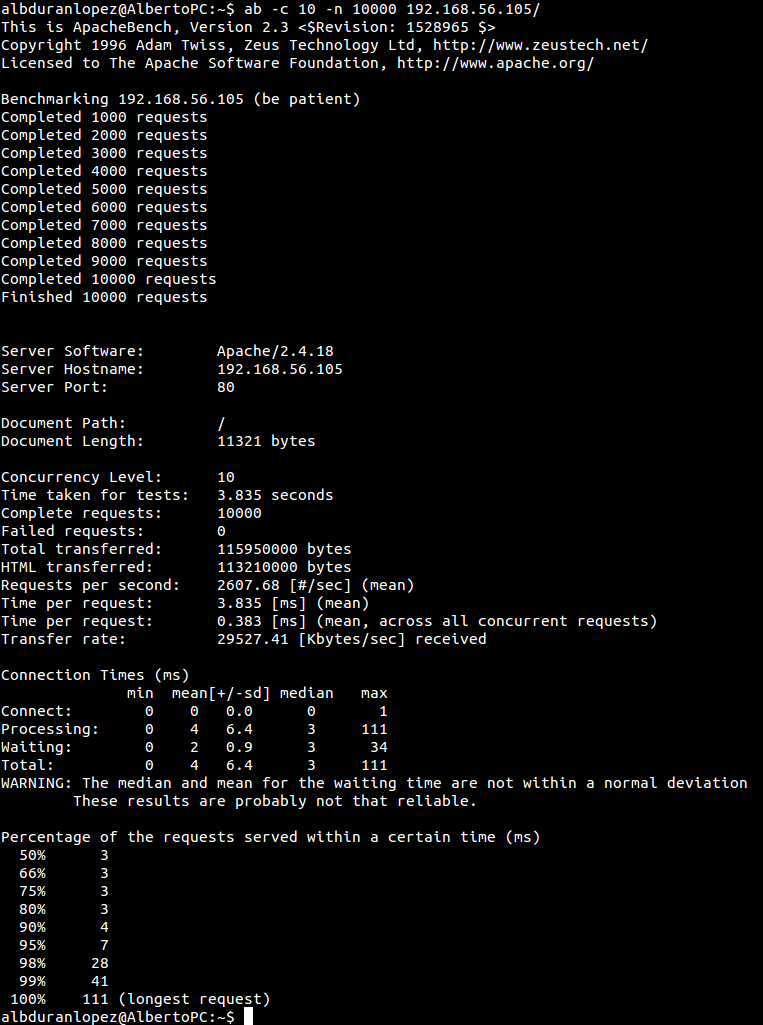
\includegraphics[scale=0.347]{images/Bubuntu.png}
		\caption{Benchmark sobre Ubuntu Server}
	\end{figure}
	
	
	\newpage
	\item Benchmark sobre centOS
	\begin{figure}[h]
		\centering
		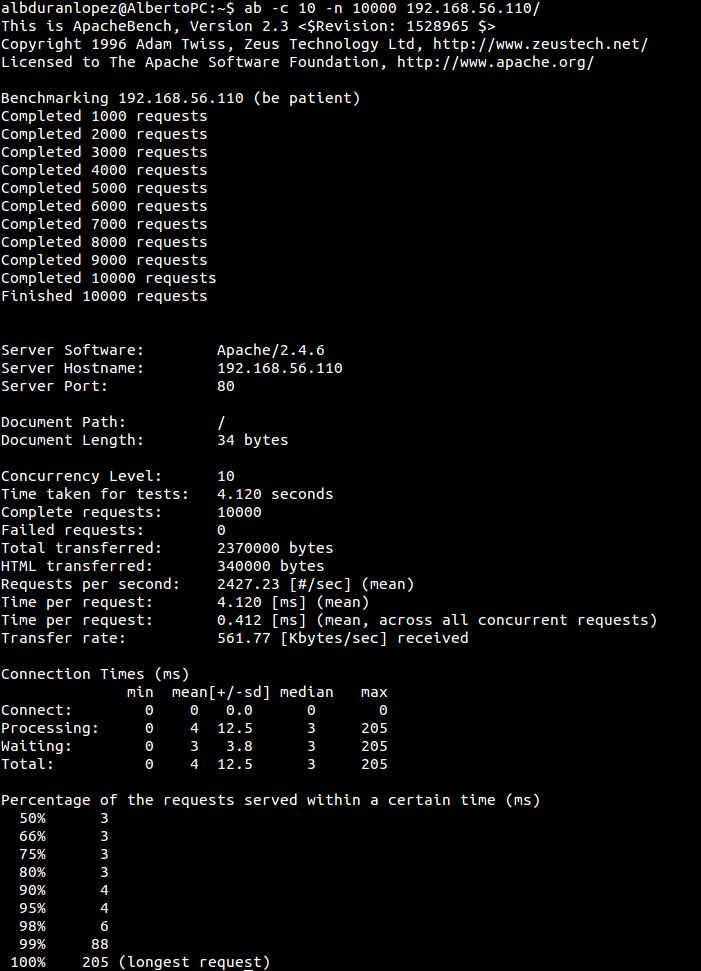
\includegraphics[scale=0.3]{images/Bcentos.png}
		\caption{Benchmark sobre centOS}
	\end{figure}
	
\end{itemize}

Como vemos en las capturas anteriores, la máquina CentOS ha consumido 4,120 segundos frente a los 3,835 segundos que ha tardado el test sobre Ubuntu. Además en Ubuntu se han transferido más bytes que en CentOS.
\begin{itemize}
	\item \textbf{Time per request}: Es menor en Ubuntu Server que en centOS
	\item \textbf{Transfer rate}: Es bastante mayor en Ubuntu que en centOS
	
\end{itemize}

En resumen, tras ejecutar el Benchmark podemos concluir que podemos obtener mejores resultados con Ubuntu Server.




\newpage
\section{Jmeter}

Es un BenchMark con funcionalidades parecidas al anterior pero algo más complejo. Este software se autodefine como una aplicación 
" \textit{designed to load test functional behavior and measure performance}".\\ Jmeter simula los \textit{N} usuarios indicados conectándose al servidor. Se caracteriza por el uso de hebras y por tener una interfaz propia. \\

Nos descargamos Jmeter con el comando:\\
\# \textit{sudo apt-get install jmeter} \\

Una vez instalado, nos conectamos mediante ssh a Ubuntu Server y ejecutamos el comando 'jmeter' para que se nos abra la interfaz

	\begin{figure}[h]
		\centering
		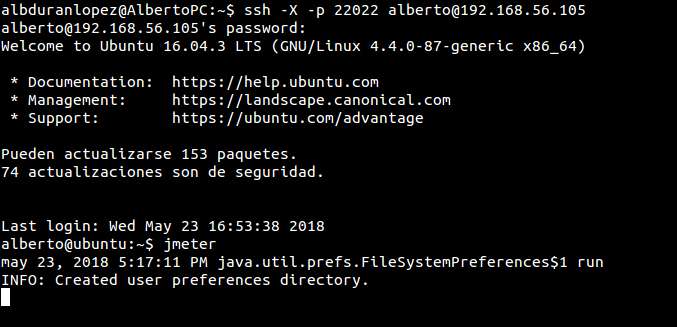
\includegraphics[scale=0.4]{images/inicioJ.png}
	\end{figure}
	
		\begin{figure}[h]
			\centering
			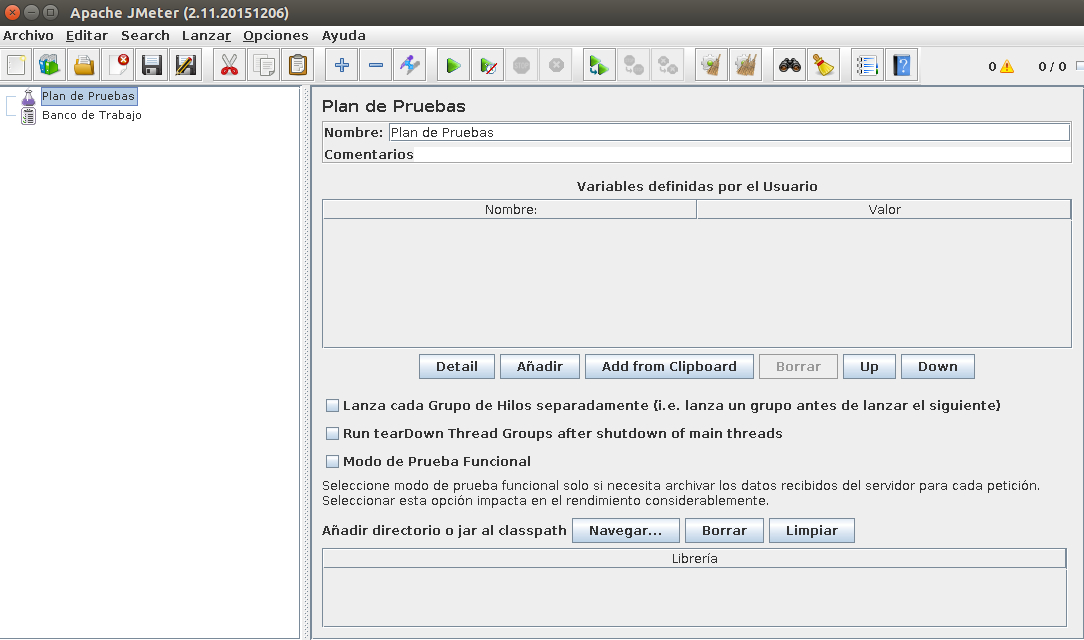
\includegraphics[scale=0.35]{images/jmeter2.png}
			\caption{Interfaz gráfica - Jmeter}
		\end{figure}
		
\newpage

Una vez hayamos iniciado JMeter, realizaremos el mismo benchmark que hemos llevado a cabo con ab para así poder comparar los resultados. Para ello tenemos que crear un \textit{Plan de pruebas} donde añadiremos el número de hilos, la concurrencia, repeticiones...etc
	\begin{figure}[h]
		\centering
		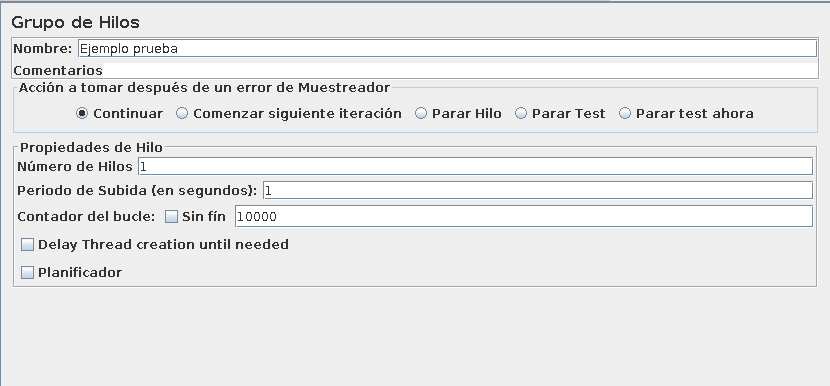
\includegraphics[scale=0.35]{images/GHJ.png}
		\caption{Grupo de Hijos - JMeter}
	\end{figure}
	
Una vez configurado el grupo de hilos, nos dirigimos al Ejemplo prueba, botón derecho:
\textit{Añadir--> Elemento de configuración-->Valores por defecto para petición HTTP} e insertamos la IP de la máquina en la que vamos a hacer las peticiones. \\ En nuestro caso, la dirección IP \textit{192.168.56.105}, la de Ubuntu Server

\begin{figure}[h]
	\centering
	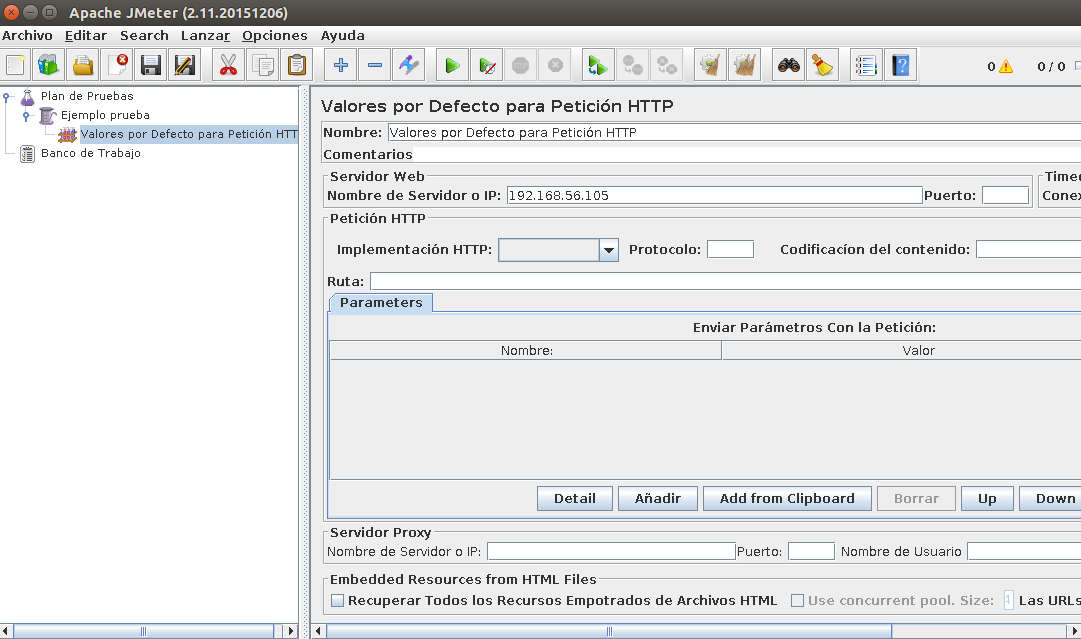
\includegraphics[scale=0.35]{images/IPJ.png}
	\caption{IP - Jmeter}
\end{figure}

\newpage
A continuación, seleccionamos la ruta de Ubuntu Server donde hacer las peticiones. 
Después le volvemos a dar en el grupo de Hijos, en nuestro caso lo hemos llamado \textit{Ejemplo prueba}:
\textit{Botón derecho-->Añadir--> Muestreador--> Petición HTTP}

En esta pestaña añadimos el nombre, en nuestro caso \textit{Apache Home} y en la ruta ponemos el directorio raíz, tal como aparece en la captura siguiente

\begin{figure}[h]
	\centering
	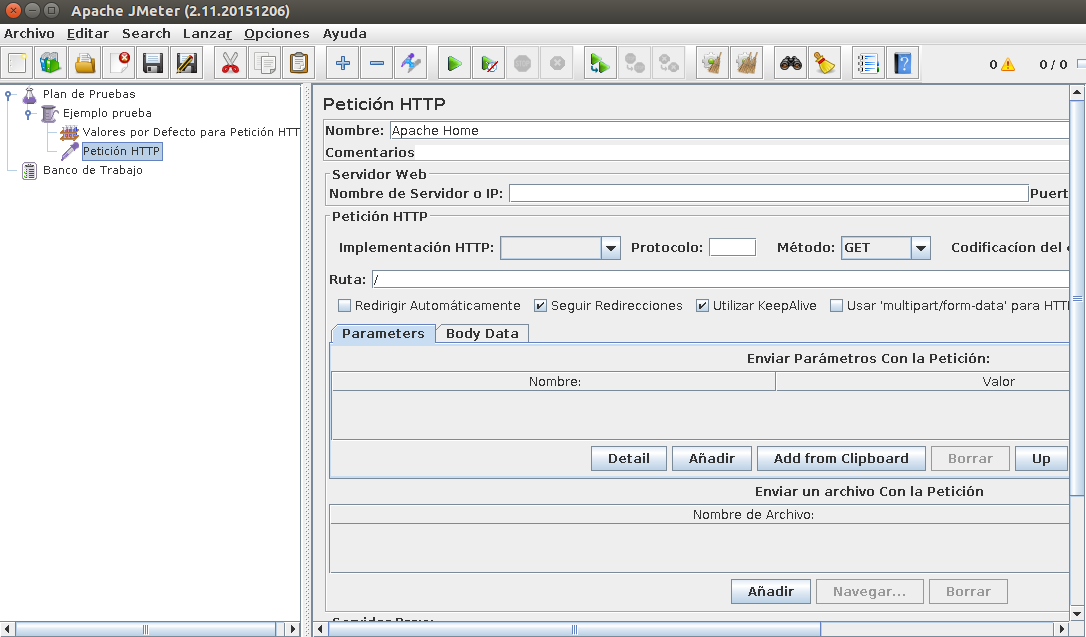
\includegraphics[scale=0.35]{images/jmeter3.png}
	\caption{Petición HTTP - Jmeter}
\end{figure}

Añadiremos una gráfica haciendo lo siguiente: \\
\begin{figure}[h]
	\centering
	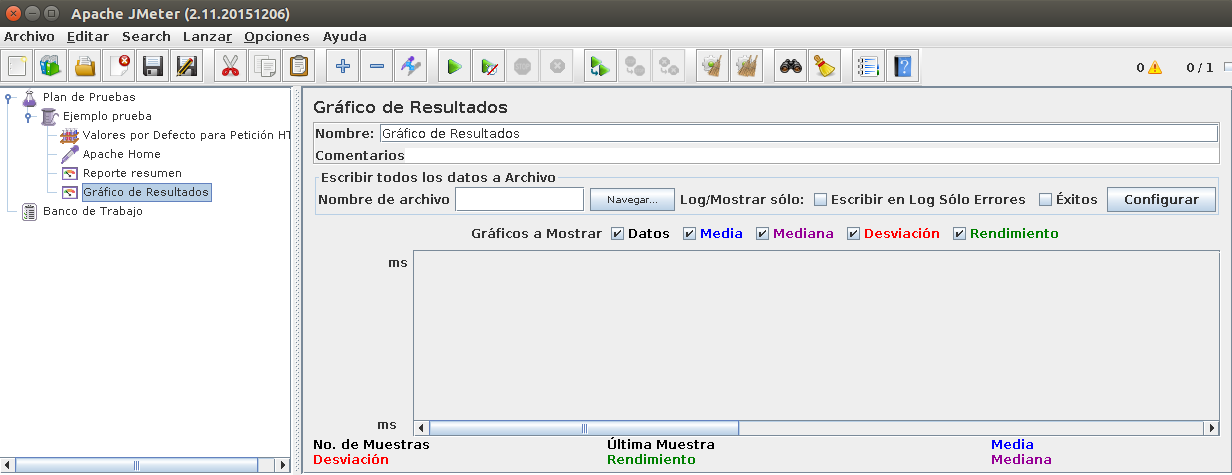
\includegraphics[scale=0.338]{images/graf.png}
	\caption{Gráfica del Benchmark}
\end{figure}


\newpage
Por último, añadimos un resumen del benchmark: \\
\textit{clic derecho sobre el grupo de hilos--> Añadir-->Receptor-->Reporte resumen} \\

Ya tenemos todo configurado, ahora arrancamos el benchmark dándole a \textit{play} y tendremos los resultados:

\begin{figure}[h]
	\centering
	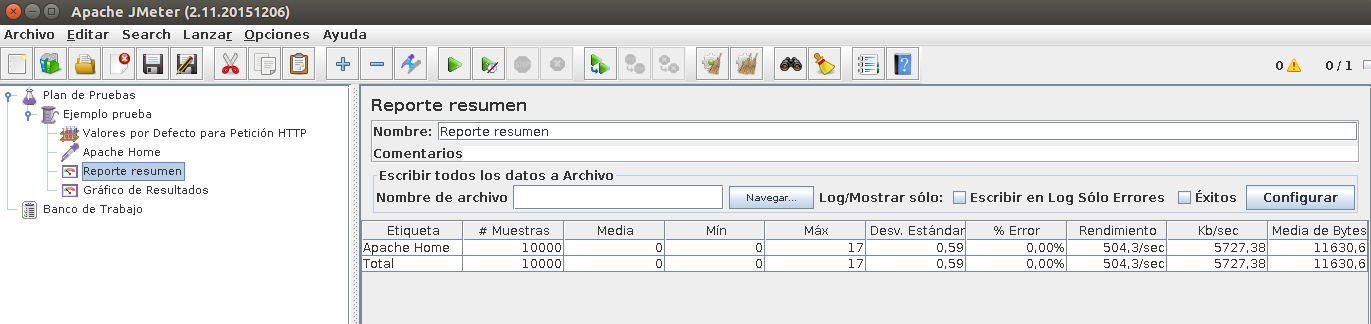
\includegraphics[scale=0.35]{images/resumen.png}
	\caption{Resumen del Benchmark}
\end{figure}

\begin{figure}[h]
	\centering
	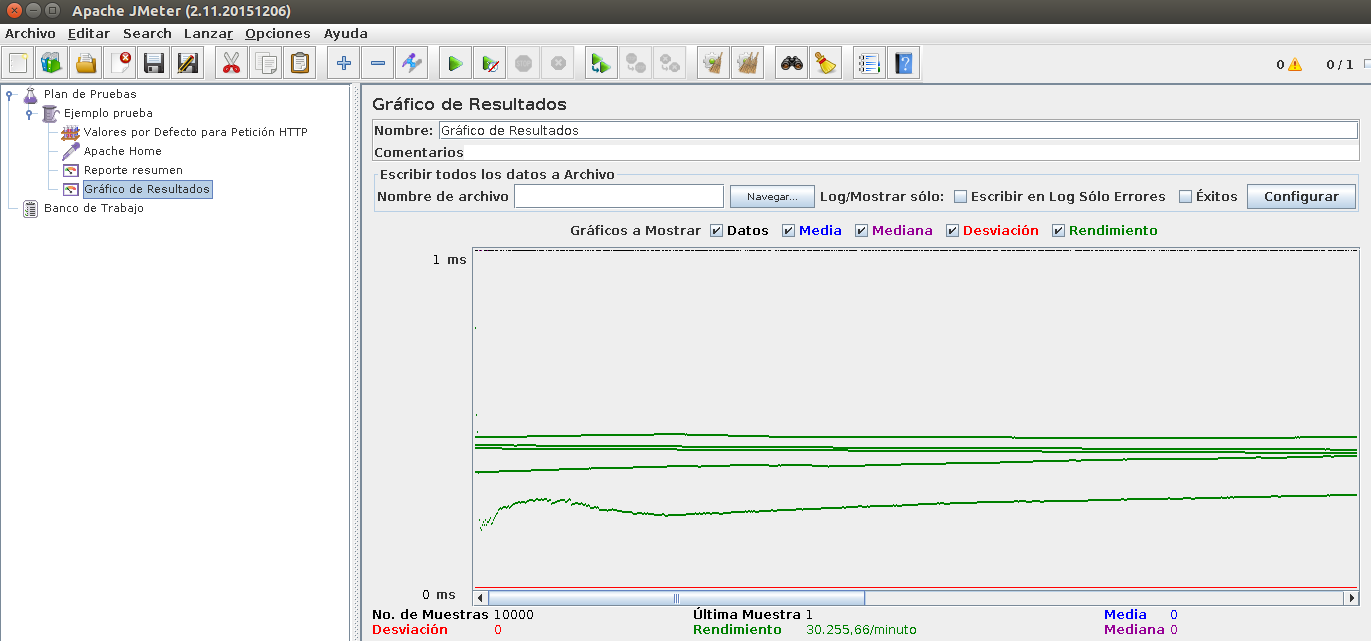
\includegraphics[scale=0.35]{images/grafico.png}
	\caption{Gráfico resultado del Benchmark}
\end{figure}

\newpage
\section*{Comparación}
Comparando la figura \textbf{3.6} y \textbf{2.1}.

Los resultados de ambos benchmark son bastante diferentes, obteniendo un mejor resultado con Apache Benchmark.
En resumen, en el test realizado con \textbf{Apache Benchmark}, teníamos 2607 peticiones por segundo y la velocidad de transferencia era de 29527 KB/sec, mientras que en JMeter tenemos 504 peticiones por segundo a una velocidad de transferencia de 5727 KB/sec 


\newpage
\section{Optimizando nuestro servidor}
El objetivo del siguiente ejercicio es el de elegir Apache, PHP o MySQL/MariaDB, modificarlo y así observar una mejora de rendimiento en el servidor. \\ Sin embargo, como ya estamos familiarizados con la pila LAMP  \textit{(Linux, Apache, MySQL/MariaDB, PHP/Python/Perl)}, intentaremos mejorar tanto Apache, PHP y MySQL

\subsection{Optimizar Apache}
En la documentación de Apache 1.3 podemos encontrar: \\

\textit{Apache es un servidor web genérico, que primero está diseñado para ser correcto, y segundo para ser rápido. Aun así, su rendimiento es bastante satisfactorio. La mayoría de los sitios web tienen menos de 10Mbits de ancho de banda de salida, que Apache puede utilizar con tan solo un servidor web que use un Pentium de gama baja.} \\

Las opciones por defecto son buenas, sin embargo, cuando la situación nos lo pide, tendremos que aplicar mejoras a nuestro servidor. Ya hemos visto varias herramientas que nos permiten monitorizar nuestro servidor, por lo que pasaremos a explicar distintas mejoras a realizar. \\
Antes de nada vamos a ejecutar algún test de Apache usando phoronix, para ello buscamos los test disponibles:

\# \textit{phoronix-test-suite list-available-tests | grep apache} \\

\begin{figure}[h]
	\centering
	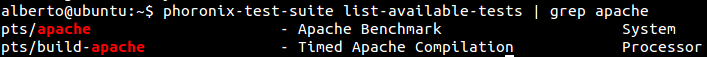
\includegraphics[scale=0.35]{images/apache122.png}
	\caption{Tests para Apache - Phoronix}
\end{figure}

\newpage
Nos descargamos un test y lo ejecutamos, los comandos a usar son los que hemos explicado al principio de la práctica.

\# \textit{phoronix-test-suite install pts/build-apache} \\

Con el comando 
\textit{phoronix-test-suite info  pts/build-php}, vemos que su métrica consiste en medir cuánto tiempo tarda en configurar el servidor HTTP. \\
\# \textit{phoronix-test-suite run pts/build-apache} \\


\begin{figure}[h]
	\centering
	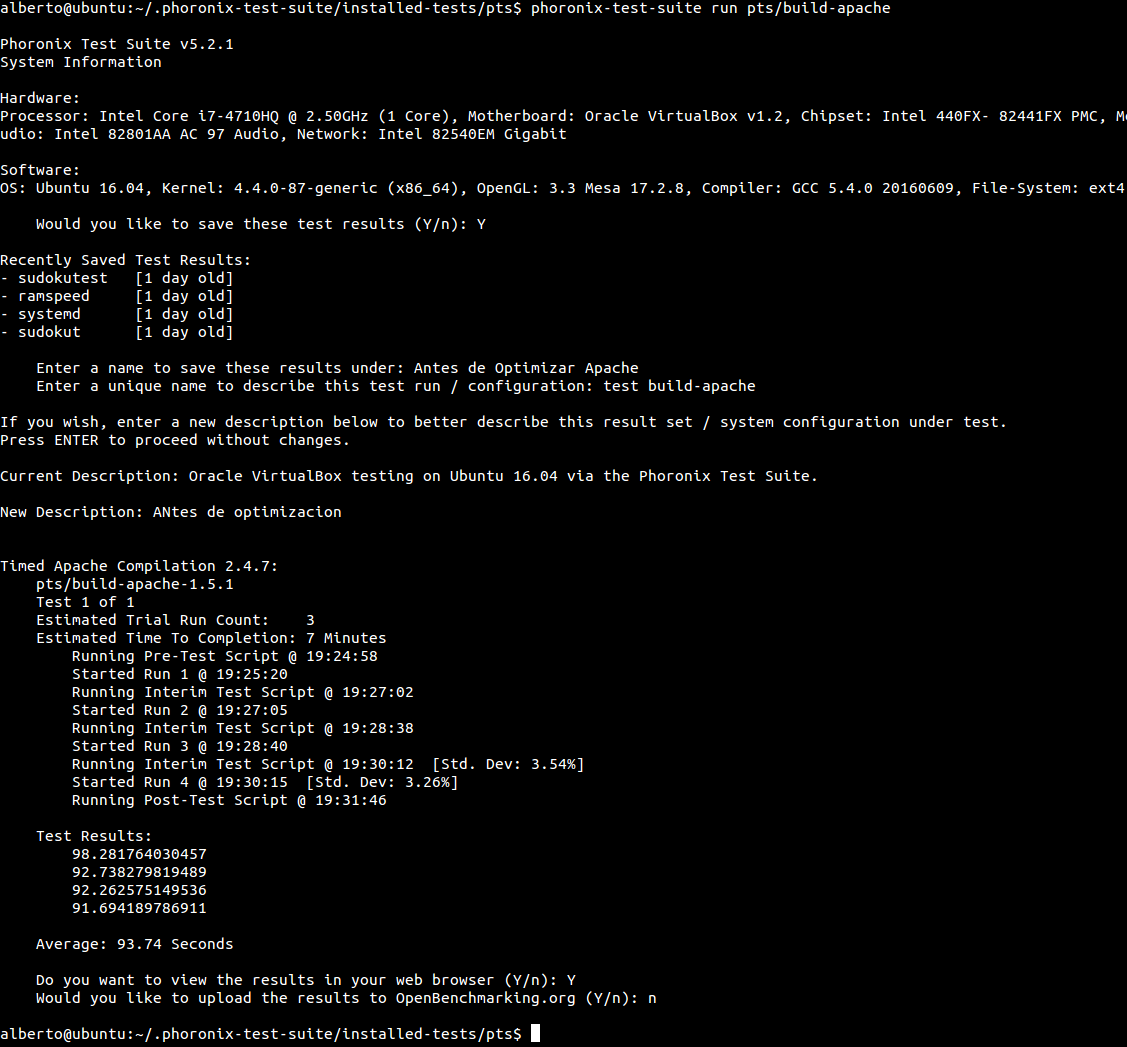
\includegraphics[scale=0.39]{images/antesOP.png}
	\caption{Ejecutando test antes de Optimizar}
\end{figure}

En el test realizado, se ejecuta el test 4 veces y se obtiene una media de casi 94 segundos. Ahora intentaremos mejorar este tiempo...

\newpage
- Continuaremos explicando que Apache tiene un registro de cada petición que recibe en sus ficheros.log de acceso. \\ 
- Escribir entradas a los ficheros de log de Apache evidentemente conlleva cierta carga, pero la información recolectada por los logs es tan valiosa que bajo circunstancias normales, el registro de logs no debe desactivarse.\\
- Hay muchas razones por las que rotar los ficheros de log ya que se hacen demasiado grandes con el tiempo, por lo que dicha rotación periódica de logs hace que el trabajo de análisis sea más manejable.  \\
- No hace falta que realicemos esta rotación manualmente, bastará con ejecutar un script desde un cron que se ejecute (dependiendo de la carga del servidor) cada semana, mes, año... \\

Vemos el tamaño de los logs de apache:
\# \textit{du -sh *} \\

\begin{figure}[h]
	\centering
	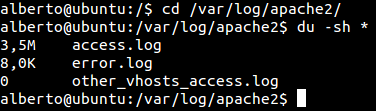
\includegraphics[scale=0.55]{images/espacio.png}
	\caption{Espacio archivos Apache}
\end{figure} 

En la captura anterior se puede ver el espacio que ocupan los diferentes ficheros aunque el archivo \textit{access.log} es el que más ocupa. Realmente 3,5 MB es poco espacio, pero... ¿y si estuviéramos ante un servidor con mucha mayor carga? \\







Por otro lado, la instalación por defecto de Apache viene con módulos instalados que seguramente no necesitemos. En Ubuntu, si nos dirigimos a \textit{/etc/apache2/mods-enabled} y a \textit{/etc/apache2/mods-available/} podemos verlos. La carpeta de mods-available es una lista de todos los módulos instalados mientras que la carpeta de mods-enabled muestra información de los módulos que están ahora mismo activos

\begin{figure}[h]
	\centering
	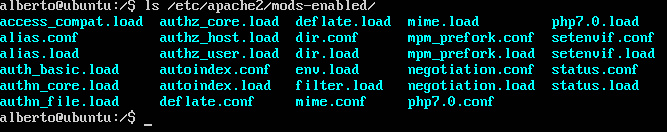
\includegraphics[scale=0.55]{images/enabled.png}
	\caption{Mods-enabled}
\end{figure} 

\newpage
Ahora bien, dependiendo de los módulos de nuestro servidor, podríamos quitar aquellos módulos que no nos interesen, para así aumentar la velocidad del servidor. \\

Para habilidad/deshabilitar módulos se hace con el siguiente comando:

\# \textit{sudo a2dismod "nombreMod"} \\
\# \textit{sudo a2enmod "nombreMod"} \\

\begin{figure}[h]
	\centering
	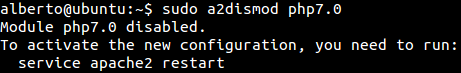
\includegraphics[scale=0.55]{images/Comandoquitar.png}
	\caption{Deshabilitar un módulo}
\end{figure} 

\begin{figure}[h]
	\centering
	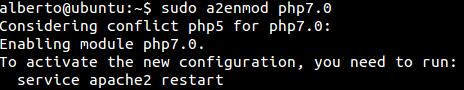
\includegraphics[scale=0.55]{images/k.png}
	\caption{Habilitar un módulo}
\end{figure} 

Para que los cambios se hagan correctamente tendremos que reiniciar el servicio\\

Entre los módulos que más consumen podemos encontrar a:
\begin{itemize}
	\item PHP
	\item SSL
	\item Rewrite
	\item Perl
	\item Python
	\item Rack / Ruby / Passenger
\end{itemize}


\newpage
Por último cuando el servidor arranca, el proceso padre arranca con un número determinado de procesos hijos/workers que hacen el trabajo de servir las peticiones recibidas. Pero dicho número de \textit{workers} se puede cambiar. Se consigue un mejor rendimiento en un servidor con un número menor de procesos pero que responda más rápido en vez de un servidor con más procesos hijos pero que no pueda responder. \\

Editamos el archivo \textit{/etc/apache2/apache2.conf} y añadimos lo siguiente:

\begin{figure}[h]
	\centering
	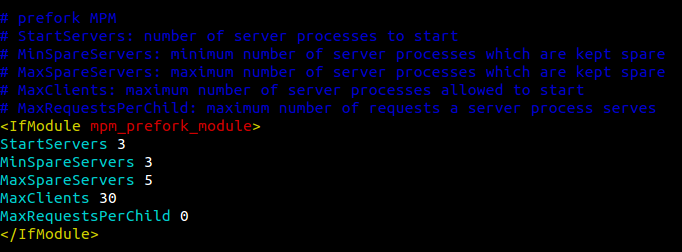
\includegraphics[scale=0.55]{images/yea.png}
	\caption{vi /etc/apache2/apache2.conf}
\end{figure} 

\begin{itemize}
	\item \textbf{StartServers}: Número de procesos con los que empieza el servidor.
	\item \textbf{MinSpareServers}: Mínimo número de procesos de servidor que se guardan de repuesto.
	\item \textbf{MaxSpareServers}: Máximo número de procesos de servidor que se guardan de repuesto.
	\item \textbf{MaxClients}: Máximo número de procesos de servidor cuyo inicio está permitido.
	\item \textbf{MaxRequestPerChild}: Número máximo de peticiones que un proceso de servidor sirve.
\end{itemize}


\newpage
Tras haber deshabilitado los módulos que no usamos y haber modificado el archivo de configuración, volvemos a reiniciar el test:

\begin{figure}[h]
	\centering
	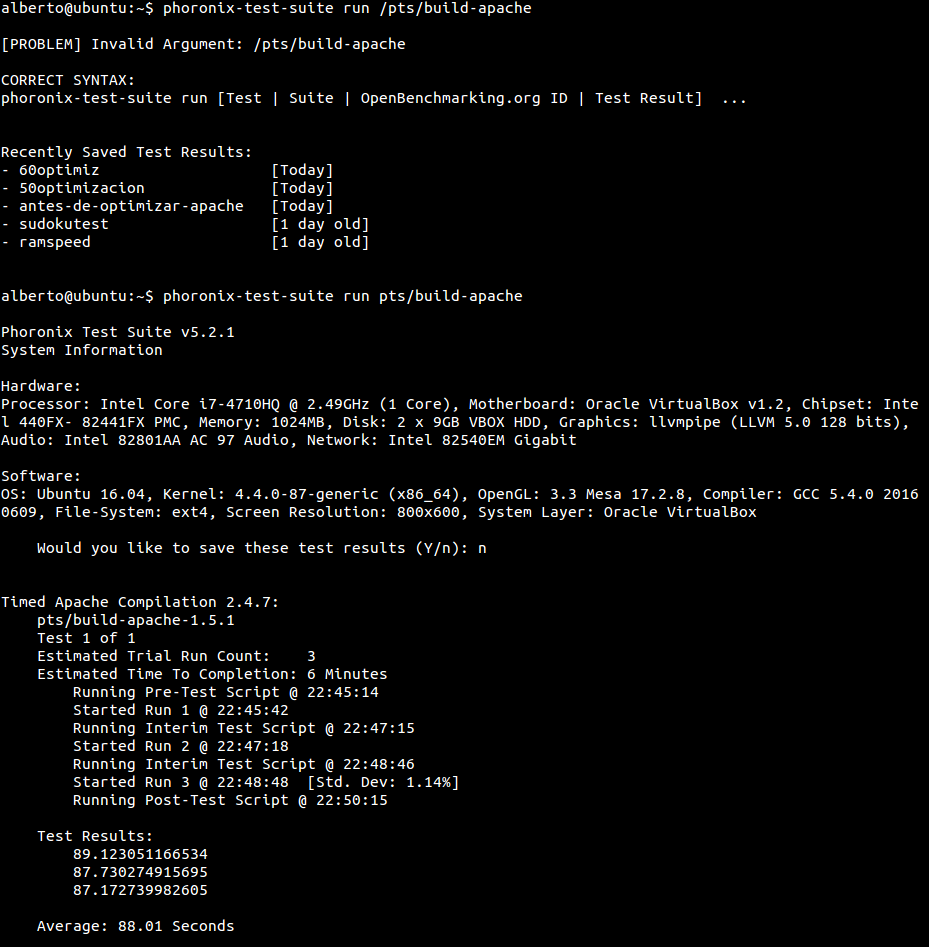
\includegraphics[scale=0.45]{images/postTest.png}
	\caption{Post-optimización - Build-Apache}
\end{figure} 

Como podemos observar, se ha reducido en unos segundos el Benchmark con respecto a la figura 4.2, en total unos 5 segundos de media. \\


\newpage
\subsection{Optimizar PHP}

Antes de empezar con la optimización de \textit{PHP}, nos descargamos un benchmark de phoronix y lo ejecutamos. El benchmark lo hemos conseguido de la forma:

\# \textit{phoronix-test-suite list-available-tests | grep php} \\
\# \textit{phoronix-test-suite install pts/build-php} \\
\# \textit{phoronix-test-suite run pts/build-php} \\

Con el comando \textit{phoronix-test-suite info pts/build-php} comprobamos que su métrica consiste en medir cuanto tiempo tarda en configurar php


\begin{figure}[h]
	\centering
	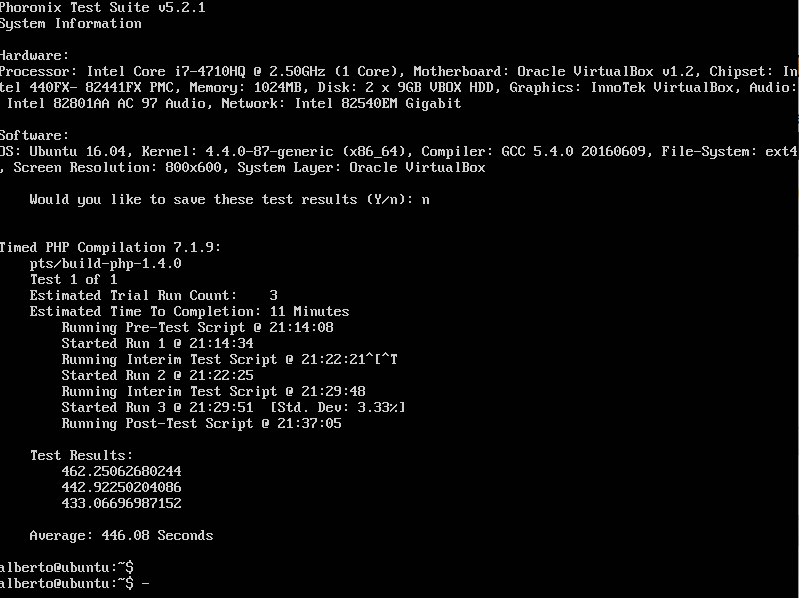
\includegraphics[scale=0.45]{images/prephp.png}
	\caption{phoronix - pts/build-php}
\end{figure} 

El benchmark se ha ejecutado 3 veces con una media de 446 segundos es decir, algo más de 7 minutos.

\newpage

Modificamos el archivo de configuración de \textit{PHP} con el siguiente comando:

\# \textit{sudo vi /etc/php/7.0/cli/php.ini} \\



\begin{figure}[h]
	\centering
	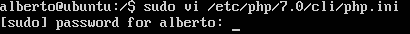
\includegraphics[scale=0.5]{images/phpini.png}
	\caption{/etc/php/7.0/cli/php.ini}
\end{figure} 

El significado de cada uno de las variables está puesta en color azul.\\ La configuración por defecto traía los valores de subida, tamaño, limite de memoria..etc bastante pobres por lo que los aumentamos.

\begin{figure}[h]
	\centering
	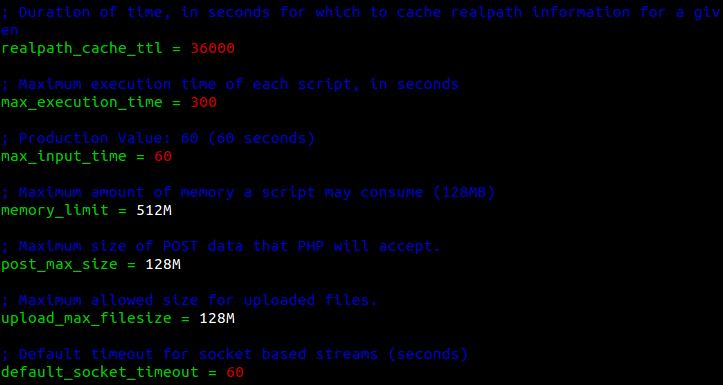
\includegraphics[scale=0.5]{images/prec.png}
	\caption{Modificando parámetros php.ini}
\end{figure} 




\newpage
Realizamos el benchmark de nuevo:

\begin{figure}[h]
	\centering
	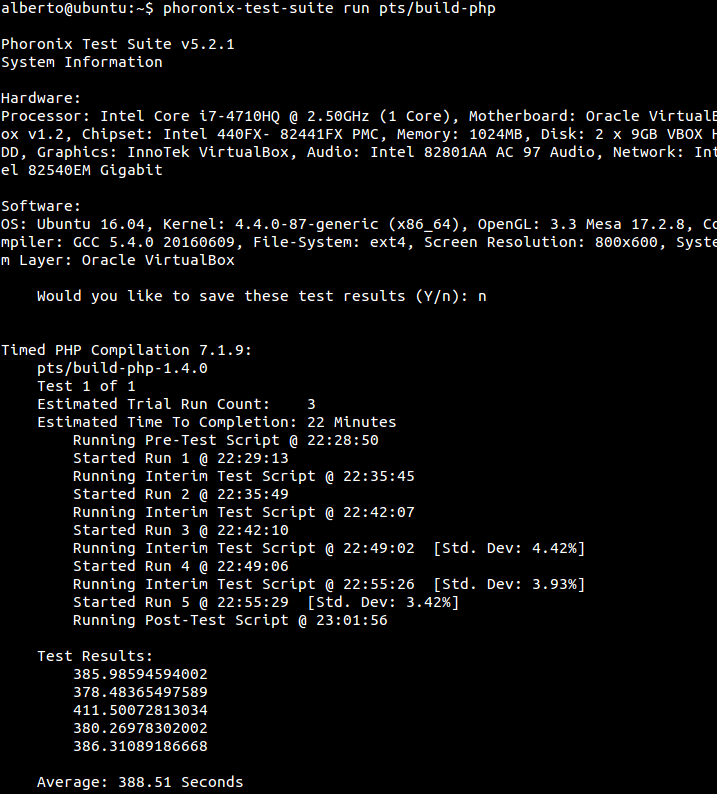
\includegraphics[scale=0.45]{images/post2.png}
	\caption{Build-php Benchmark}
\end{figure} 
Tras realizar la mejora, volvemos a realizar el mismo benchmark sobre php y vemos que esta vez se ha realizado 5 veces pero la media es de 388 segundos. Es decir, se ha reducido bastante el tiempo frente al tiempo obtenido en la figura 4.9, un total de casi 60 segundos de mejora. \\




\newpage
\subsection{Optimizar MySQL}

Para intentar realizar un benchmark sobre MySQL, he buscado en phoronix pero no he encontrado ninguno :(

\begin{figure}[h]
	\centering
	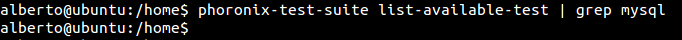
\includegraphics[scale=0.35]{images/noresult.png}
	\caption{phoronix - no MySQL tests}
\end{figure} 

Ejecutando el siguiente comando, vemos que tenemos disponible el siguiente benchmark, también disponible en \url{https://dev.mysql.com/doc/refman/5.5/en/select-benchmarking.html} \\
\# \textit{sudo apt-cache search mysql | grep benchmark} \\


\begin{figure}[h]
	\centering
	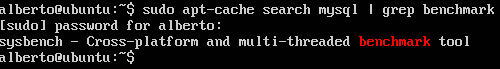
\includegraphics[scale=0.5]{images/sysbench1.png}
	\caption{SysBench - MySQL}
\end{figure} 

Con ayuda del manual, \textit{man}, podemos ver las diferentes opciones que tiene.

Una vez instalado, creamos una base de datos: \\

\# \textit{mysql -uroot -ppracticas,ISE -e ''create database dbbench''} \\

Una vez creada, preparamos el test creando una nueva tabla básica: \\

\# \textit{sysbench $--$test=oltp $--$oltp=table-size=<numero de filas> $--$mysql-db=dbbench $--$mysql-user=root $--$mysql-password=<password> prepare} \\


\begin{figure}[h]
	\centering
	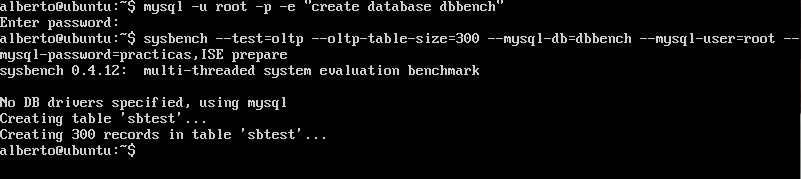
\includegraphics[scale=0.5]{images/sysbench3.png}
	\caption{SysBench - MySQL}
\end{figure}

\newpage
Para ejecutar el test, realizamos lo siguiente:

\# \textit{sysbench $--$test=oltp $--$oltp=table-size=<numero de filas> $--$oltp-test-mode=complex $--$num-threads=<numero de hebras> $--$max-time=60 $--$max--mysql-db=dbbench $--$mysql-user=root $--$mysql-password=<password> run} \\

En nuestro caso hemos determinado a 300 el número de filas y a 10 el nº de hebras.

\begin{figure}[h]
	\centering
	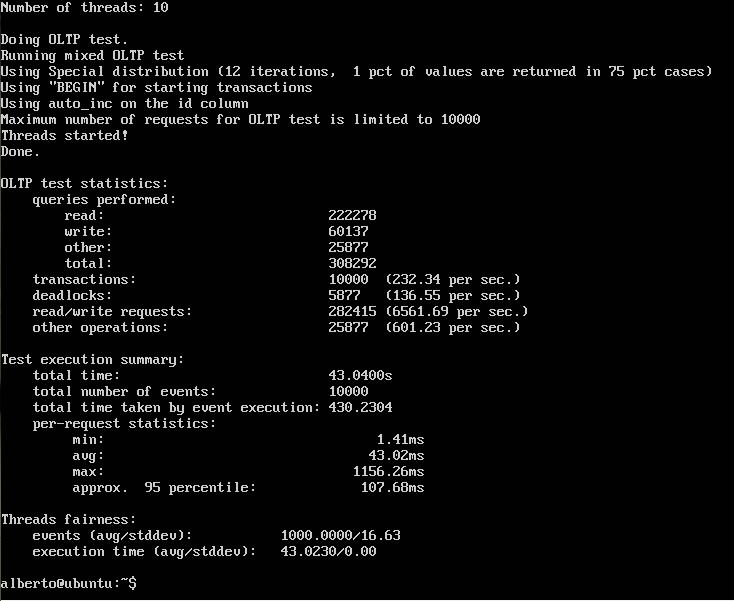
\includegraphics[scale=0.5]{images/antes.png}
	\caption{SysBench - Antes de la mejora}
\end{figure}

Como podemos observar en la imagen anterior, se realizan una serie de lecturas y escrituras, obteniendo un tiempo total de 43 segundos en su ejecución.

\newpage

Nos disponemos a realizar la mejora:

Nos descargamos \textit{mysqltuner}, un programa que se ejecuta en nuestra máquina, nos evalúa la configuración de MySQL y nos recomienda hacer mejoras sobre ésta. \\
Nos lo descargamos e iniciamos con: \\
\# \textit{sudo apt-get install mysqltuner} \\


\begin{figure}[h]
	\centering
	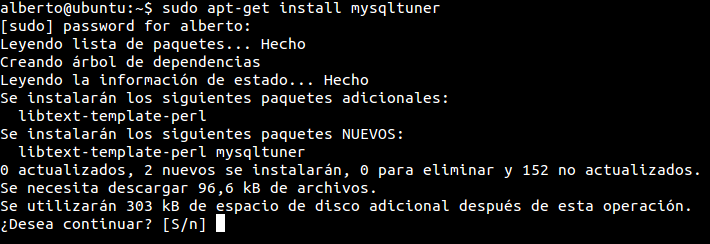
\includegraphics[scale=0.5]{images/mysqlTuner.png}
	\caption{vi /etc/apache2/apache2.conf}
\end{figure} 

Ejecutamos el comando: \\
\# \textit{mysqltuner} \\

\begin{figure}[h]
	\centering
	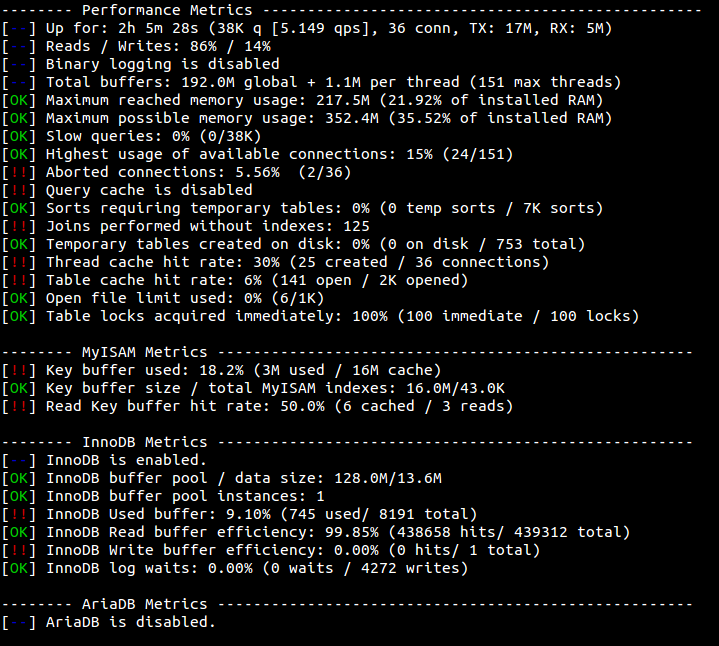
\includegraphics[scale=0.4]{images/mysql.png}
\end{figure} 

\begin{figure}[h]
	\centering
	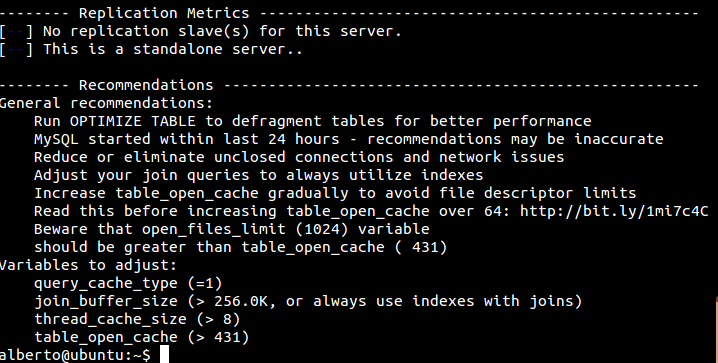
\includegraphics[scale=0.4]{images/mysqltuner2.png}
	\caption{mysqltuner}
\end{figure}

\newpage
Como vemos en la captura anterior, en \textit{Recommendations} podemos observar que nos ofrece unas recomendaciones generales así como una variables que tenemos que ajustar para mejorar la configuración. Por lo que nos dirigimos al archivo de configuración de \textit{mysql}, \textit{/etc/mysql/mysql.conf.d} y lo editamos.

\# \textit{sudo vi /etc/mysql/mysql.conf.d/mysqld.cnf } \\

\begin{figure}[h]
	\centering
	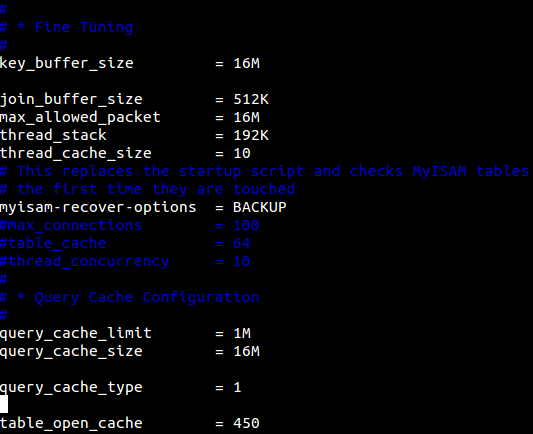
\includegraphics[scale=0.5]{images/weno.png}
	\caption{/etc/mysql/mysql.conf.d/mysqld.cnf}
\end{figure}


\newpage
Reiniciamos el servicio para que los cambios tengan efecto: \\
\# \textit{systemctl restart mysql} \\



\begin{figure}[h]
	\centering
	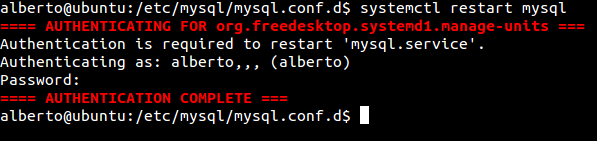
\includegraphics[scale=0.4]{images/restart.png}
	\caption{Reiniciando mysql.service}
\end{figure} 



Una vez ya realizada la mejora de nuestro MySQL, realizamos el benchmark \textit{sysbench} anterior:

\begin{figure}[h]
	\centering
	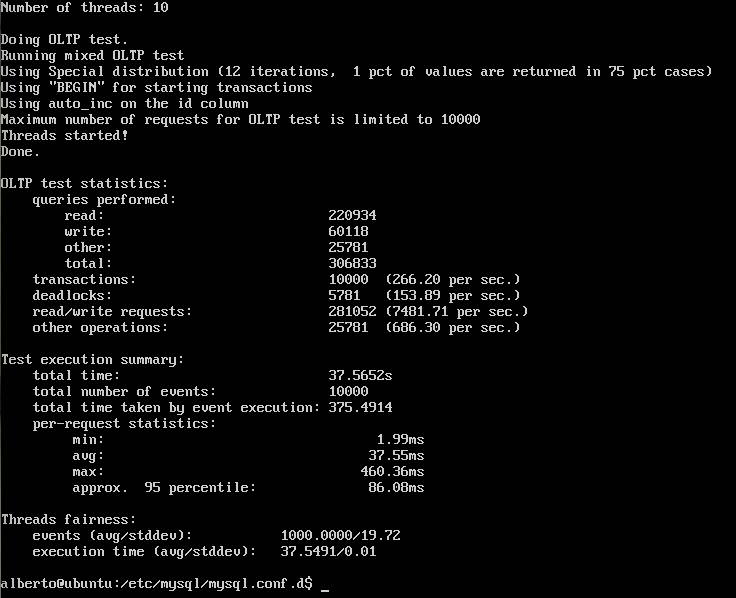
\includegraphics[scale=0.44]{images/despu.png}
	\caption{sysbench - Después de la mejora}
\end{figure} 


Tras realizar el mismo test que hemos realizado anteriormente obtenemos una mejora en el tiempo de ejecución de este.
Frente a los resultados de la figura \textbf{4.16} hemos conseguido que mysql reduzca su ejecución del benchmark a 37,5 segundos. \\


Si observamos la Figura \textbf{4.18}, otras recomendaciones que nos ofrecen son las de optimizar las tablas con el comando \textit{OPTIMIZE TABLE} (para desfragmentar las tablas) y así obtendríamos un mejor rendimiento. 





\newpage
\begin{thebibliography}{9}
	
	\bibitem{Apache Documentation} 
	Apache Documentation,
	\\\texttt{https://httpd.apache.org/docs/2.4/programs/ab.html}
	
	\bibitem{Apache Documentation} 
	Apache Documentation,
	\\\texttt{https://httpd.apache.org/docs/trunk/es/misc/perf-scaling.html}
	
	\bibitem{Digital Ocean} 
	Digital Ocean,
	\\\texttt{https://www.digitalocean.com/community/tutorials/how-to-optimize-apache-web-server-performance}
	
	\bibitem{Rudd-o} 
	Rudd-o,
	\\\texttt{https://rudd-o.com/linux-and-free-software/tuning-an-apache-server-in-5-minute}
	
	\bibitem{Apache} 
	Apache,
	\\\texttt{https://www.garron.me/es/gnu-linux/apache-php-fpm-mpm-worker-mariadb-ubuntu.html}
	
	\bibitem{Apache} 
	Apache,
	\\\texttt{http://www.webhostingtalk.com/showthread.php?t=661905}
	
	\bibitem{Apache} 
	Apache,
	\\\texttt{https://dev.mysql.com/doc/refman/5.5/en/select-benchmarking.html}
	
	\bibitem{MySQL} 
	MySQL,
	\\\texttt{	http://blog.flux7.com/blogs/benchmarks/using-sysbench-to-benchmark-mysql}
	
	
	\bibitem{MySQL} 
	MySQL,
	\\\texttt{	http://blog.flux7.com/blogs/benchmarks/using-sysbench-to-benchmark-mysql}
	
	

	
	\bibitem{Tune LAMP-Server} 
	LAMP server,
	\\\texttt{https://blog.udacity.com/2015/03/optimizing-fine-tuning-lamp-server.html}
	
	
	
	\bibitem{MySQL} 
	MySQL,
	\\\texttt{https://dev.mysql.com/doc/refman/5.5/en/select-benchmarking.html}
	\\
	
	
\end{thebibliography}


\end{document}